\documentclass{standalone}
\usepackage{tikz}
\usepackage{mathrsfs}
\usetikzlibrary{positioning, shapes.geometric, arrows}
\usepackage[T1]{fontenc}
\renewcommand*\familydefault{\ttdefault} %% Only if the base font of the document is to be typewriter style
\begin{document}
	 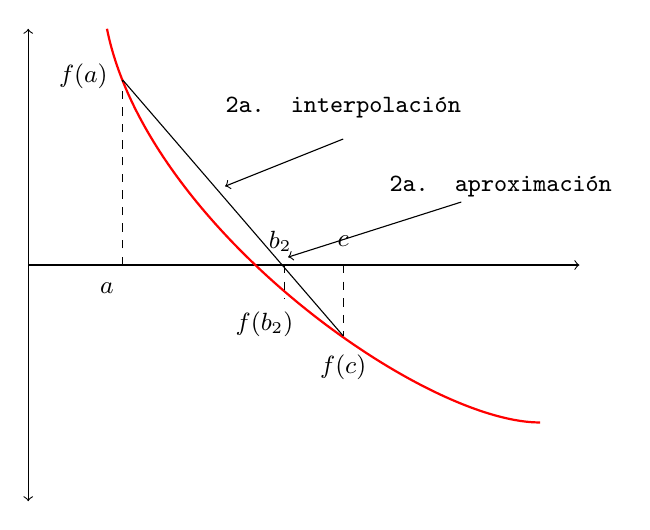
\begin{tikzpicture}[font=\small]
		\draw [->] (0,0) -- (7,0);
		\draw [<->] (0,-3) -- (0,3);
		\draw [red, thick] (1,3) .. controls (1.5,0.5) and (5,-2) .. (6.5,-2);
		\draw (1,-0.3) node {$a$};
		\draw (0.7, 2.4) node {$f(a)$};
		\draw (4,0.3) node {$c$};
		\draw (4, -1.3) node {$f(c)$};
		\draw [dashed] (4,0) -- (4,-0.9);
		\draw [dashed] (1.2,0) -- (1.2,2.35);\pause
		\draw (1.2,2.35) -- (4,-0.9);
		\draw  (4,2) node {2a. interpolación};
		\draw [->] (4,1.6) -- (2.5,1);\pause
		\draw [dashed] (3.25,0) -- (3.25,-0.43);
		\draw (3.2, 0.3) node {$b_{2}$};
		\draw (3, -0.75) node {$f(b_{2})$};
		\draw  (6,1) node {2a. aproximación};
		\draw [->] (5.5,0.8) -- (3.3,0.1);
	\end{tikzpicture}
\end{document}